\documentclass{csfourzero}
\title{Choosing taxicab fare prices using a Q-Learner}
\author{Karlis Venters}
\date{\today}

\usepackage{algorithm}
\usepackage{algpseudocode}

\usepackage[backend=biber,
            style=authoryear,
            texencoding=utf8,
            bibencoding=utf8]
  {biblatex}
\addbibresource{../literature/ai.bib}
\addbibresource{../literature/general.bib}
\addbibresource{../literature/taxi.bib}
\addbibresource{../literature/technologies.bib}

\usepackage{color}

\usepackage{hyperref}
\makeatletter
\hypersetup{
  bookmarks=true,
  pdftitle={\@title},
  pdfauthor={\@author},
  pdfsubject={Computer Science Level 4 Honours Project at University of Aberdeen},
  pdfkeywords={reinforcement learning} {q-learning} {ruby} {taxi economics} {variable pricing},
  pdfnewwindow=true,      % links in new window
  colorlinks=false,       % false: boxed links; true: colored links
  linkcolor=red,          % color of internal links (change box color with linkbordercolor)
  citecolor=green,        % color of links to bibliography
  filecolor=magenta,      % color of file links
  urlcolor=cyan           % color of external links
}
\makeatother

\usepackage{pdfpages}
\usepackage{url}

\setcounter{secnumdepth}{3}
\setcounter{tocdepth}{3}

\newcommand{\todo}[1]{\textcolor{red}{@TODO: #1}}

\begin{document}

\todo{check spelling in all files}
\maketitle

\pagenumbering{roman}

\newpage
\section*{Declaration}
\addcontentsline{toc}{section}{Declaration}

I declare that this document and the accompanying code has been composed by
myself, and describes my own work, unless otherwise acknowledged in the text.
It has not been accepted in any previous application for a degree. All verbatim
extracts have been distinguished by quotation marks, and all sources of
information have been specifically acknowledged.\\[5ex]

Karlis Venters \\[3ex]

Date: \today \\[3ex]


\newpage
\section*{Abstract}
\addcontentsline{toc}{section}{Abstract}
\begin{abstract}~

Taxi fare regulation and fixed taxi fare prices are inefficient. This project
suggests a variable fare pricing approach fo improve taxi profitability, where
the prices are chosen using reinforcement learning. Specialised simulation
software called Taxi-sim was developed for this project and published online.
The user of Taxi-sim can specify environmental constraints and market
characteristics, and taxi agents in the simulation are operated by a simple
Q-Learner. The experimental simulation results show that the Q-Learner was able
to improve its profit over time when using variable fare pricing, and that its
profits were significantly larger than when it used fixed fare pricing.
However, the analysis of fixed pricing data showed no profitability and no
profitability improvement over time, either suggesting that the Q-Learner is
not suitable for fixed pricing or revealing an implementation bug. This project
concludes that reinfiorcement learning can successfully be used for setting
taxi fare prices and justifies further study in the field. Some of the future
work can be done using the Taxi-sim simulation software which has been designed
to be modular and extensible, however it is important to be aware of its
limitations and known bugs.

\end{abstract}


\newpage
\section*{Acknowledgements}
\addcontentsline{toc}{section}{Acknowledgements}

I would like to thank my supervisor Dr. Nir Oren for all the advice and
assistance he provided over the course of the project.

I would also like to thank the people who advised me and helped with
proofreading the report.


\newpage
\addcontentsline{toc}{section}{Table of Contents}
\tableofcontents{}

\newpage
\addcontentsline{toc}{section}{List of Figures}
\listoffigures

\newpage
\pagenumbering{arabic}
(10, for the whole of report)

Is the writing clear, concise, and with good English and no typos? Is it easy
to understand the student’s explanation?

Is the dissertation sensibly structured into chapters and sections?

Is the dissertation of an appropriate length?

Are diagrams and tables useful and used adequately (referred to in the text and
explained)?

Do references to literature and URL’s follow a standard? Are they consistent?

Overall: Is the dissertation as a document of a high standard, appropriate for
a first/second/third class degree?

\subsection{Overview}

Taxicabs often use taximeters to calculate their fares based on route distance
and time spent travelling. However, the actual costs and potential profits are
influenced by more factors. If fare prices were set dynamically, they would
account for the actual environment and increase profitability of taxicabs.
Usage of artificial intelligence (AI) has been successfully researched in
\cite{tavares2012reinforcement} and \cite{ben2010road} for traffic routing, and
in \cite{lou2011optimal} for variable pricing of toll lanes. A variable pricing
approach for public transport fares is suggested in \cite{emele2013agent}.
Therefore AI could be used to dynamically price taxicab fares.


\paragraph{}
This is where it all starts.

\subsection{Taxis}
Taxis (also known as \textit{taxicabs}) are an important part of public transportation. Because of their prevalence worldwide and importance in transportation a wide range of literature has been produced on taxis. For this project, the most relevant area of this literature is economical modelling of taxi markets, an overview of which is given by \textcite{Salanova2011taxi+review}. A major topic in the research and discussion on taxis is taxi market regulation, and parts of it are relevant and will be considered in some detail. Three different taxi markets can be distinguished: cruising taxi market when a passenger hails the taxi no the street, phone-order taxi market, and taxi ranks where multiple taxis wait for passengers.
\paragraph{}Regulation is a sensitive topic for taxi research as no general consensus has been reached on whether it is recommended. \textcite{Cairns1996taxi+competition} investigated economic workings of taxi markets and incorporated results of earlier research in their economic equilibria findings. They concluded that regulation is needed to achieve non-negative profits (the so-called economic second best). \textcite{Oecd2007taxi+policy}, cited by \textcite{Salanova2011taxi+review} lists arguments both for and against regulation as observed in different countries, and notes that markets with widely varying regulation can operate successfully. SHOULD THIS BE HERE? ==>> The approach suggested by this project is not compatible with a market where fares are regulated, at least in the current form of regulation that specifies a formula to calculate fares based on some variables, usually time and distance. Other ways of regulation, for example, entry conditions, are compatible with the suggested approach and do not require any further investigation. It is important to note that some markets considered \textit{deregulated} still have some form of fare regulation, for example, taxis in New Zealand are required to list their maximum fares based on time and distance \parencite{Gaunt1995taxi+newzealand}, but are not forced to follow them.
\paragraph{}Taxi market modelling was first done by \textcite{Douglas1972taxi+regulation} according to \textcite{Salanova2011taxi+review}. He investigated a regulated cruising-taxi market (where a customer hails a taxi on the street on visual contact) and defined the fundamental taxi problem to be finding an equilibrum of an optimal level of service matching an optimal price. His limited model has been used as reference by all the later authors cited by \textcite{Salanova2011taxi+review} that have extended it to other taxi markets and factored in more environmental influences. \textcite{Devany1975taxi+capacity} researched regulated taxi markets organised as a franchised monopoly, using a medallion system, and having free entry, having the goal of finding equilibrium output, capacity and utilisation. He gave a formula tor passenger demand depending on taxi fare, passenger value of time and waiting time. \textcite{Manski1967taxi+demand} analyse the taxi market from a purely economical point of view and conclude that in addition to exogenous variables, passenger demand for taxi services is also directly related to taxi supply through waiting time. Similarly, taxi supply is influenced by taxi utilisation, which in turn directly depends on passenger demand.
\paragraph{}The most recent publications are sophisticated models based on the network model for cruising-taxi market by \textcite{Yang1998taxi+network}. This network was modelled as a graph and assumed constant taxi demand and supply, passenger demand was represented as origin-destination matrices. Finally, this paper suggested an algorithm to find an equilibrum for the optimal number of taxis in a market and equations to calculate taxi utilisation and customer waiting time. In contrast, \textcite{Yang2000taxi+utilization} focuses on supply and demand to recommend optimal policies for taxi regulation in Hong Kong and base their model on various data sources. A number of exogenous and endogenous variables affecting taxi market are identified, and equations are suggested to calculate them: passenger waiting time, percentage of occupied taxis, vacant taxi headway, daily taxi passenger trips and taxi waiting time. This model can be used to forecast taxi demand, taxi utilization and service quality, although the authors warn that it does not take in account the complex supply-demand relationships in taxi market.
\paragraph{}Consequently \textcite{Yang2002taxi+demand} continued to evaluate the supply-demand equilibria of taxi market started by \textcite{Yang1998taxi+network} and \textcite{Yang2000taxi+utilization}, resulting in the conclusion that the spatial characteristics of a network where taxis are operating strongly influence supply, demand and should bear weight when evaluating regulatory policies.This study focuses on social surplus (the sum of customer surplus and producer surplus) as the key objective of taxi markets. Four different regulatory frameworks that could be applied to taxi markets are investigated: free entry and unconstrained fare, free entry and regulated fare, regulated entry and unconstrained fare, and regulated entry and regulated fare. All of these cases are investigated with both competitive and monopilistic markets, and equilibria are found.
\paragraph{}
\textcite{Wong2008taxi+modeling} extended this model to heterogenous vehicle and user classes, and included congestion which is a major issue in reality particularly in big cities, but was ignored by most of earlier research. The way how cruising taxis and customers find each other was researched by \textcite{Yang2010taxi+equilibria}, paying particular attention to customer behaviour. \textcite{Yang2010taxi+nonlinear} proposes a nonlinear fare structure to correct market and regulatory inefficiencies, and applies it to a similar model.


\subsection{Reinforcement learning}

\newpage
\section{Requirements}
\label{sec:requirements}

\todo{remove note}
(5, 1000w)

Has the student appropriately analysed and defined the requirements for the
project and presented them clearly?


\subsection{Functional Requirements}
\label{sec:requirements:simulation}

The following requirements are derived directly from the project's goals set in
Section \ref{sec:intro:goals}. Alas, it is unfeasible to structure this section
around each goal as they contain several requrements that sometimes overlap
with other goals. Each of the following requirement categories is discussed in
detail, listing what could be implemented in the best case scenario without any
time pressure. However, to stay realistic and make sure that core functional
requirements are prioritised, the minimal requirements are separately summed up
in Table \ref{table:requirements} for each of the following sections.


\subsubsection{Market Considerations}

The approach suggested by this project is not compatible with a market where
fares are regulated, at least in the current form of regulation that specifies
a formula to calculate fares based on some variables, usually time and
distance. Other ways of regulation that do not affect pricing, for example,
market entry conditions, are compatible with the suggested variable pricing
approach.

Three different operational types of taxi markets were introduced in Section
\ref{sec:literature:taxis}: phone-order market, cruising taxi market and taxi
rank market. In the phone-order market and taxi rank customers are actively
seeking a taxi, while in the cruising taxi market passengers can only wait for
a taxi to drive by. Therefore the cruising taxi market is chosen as the easiest
target for simulation, extending it to phone-order and taxi rank markets if the
initial experiment is successful.

The relationship between taxi demand and supply and vice versa was established
in Section \ref{sec:literature:taxis:demand}. This relationship largely depends
on the competitive situation in a taxi market. This is a very complex
relationship and thus implementing it in software would require considerable
effort. Because the core goal of the project is comparing variable pricing
approaches, not correctly modelling the market, this problem can be avoided by
assuming a constant demand. Furthermore, if the environment is fixed, the
simulation only needs to support a single taxi at the very least. As the design
is planned modular, the variable demand can be factored in later when
necessary.


\subsubsection{Demand: Modelling Passengers}
\label{sec:requirements:passenger}

Customer demand was reviewed in Section \ref{sec:literature:taxis:demand} where
two approaches to modelling demand were shown: aggregate and disaggregate. An
aggregate demand model "for some portion of the travel market is a function of
variables that describe the product or its consumers"
\parencite{Small2007taxi+urban} The disaggregate approach specifies a set of
variables for each individual passenger. The project goal is investigating taxi
pricing on an individual basis, therefore an agent-based approach is
preferrable as it allows individual modelling of passengers. Of course, to
express demand as a single variable it needs to be an aggregation of the
relevant individual variables.

Therefore each passenger's demand is a function that of some variables. The
different types of variables affecting taxi demand were discussed in Section
\ref{sec:literature:taxis:demand}. Exogenous demand variables are value of time
and value of reliability that can be derived from a passenger's income, hour of
day when travelling, purpose of travel, social status, cost of waiting and
others; these can be modelled for each individual passenger. Taxi availability
is a variable directly depending on the number of vacant taxis in an area, this
is something that passenger's perceive in reality. However, for the simulation,
taxi availability needs to be assumed a constant, at least until machine
learning capabilities are added to passengers and a competitive market
established beyond the very basic simulation, so that passanger agents can
learn the availability on their own.

Let \(P\) be the set of relevant characteristic variables \(c_1,..,c_n\) for a
passenger: \(P = \{c_1,..,c_n\}\), \newline
where each \(c_i : i \in \{1, .., n\}\) has a function \(f_i (c_i) \) that
returns a unity-based normalised value of \(c_i\), \newline
and each \(c_i\) has a weight \(w_i\) representing its relative importance
compared to other variables, where \(\sum_{i=1}^n (w_i) = 1 \). \newline
Then the total probablilstic value \(V(P)\) of a passenger is \[ V(P) =
\sum_{i=1}^{n} (w_i \cdot f_i(c_i) )) \] \newline

Let \(\Delta(o,d)\) be the distance between origin \(o\) to destination \(d\). 
\newline
Let the passenger's expected fare \(F_{expect}\) linearly depend on distance
and a set price \(p\) for a unit of distance. \(F_{expect} = \Delta(o,d) \cdot
p \). \newline
Let the price sensitivity of customers be \(\frac{F_{expect}}{F_{offer}}\). It
is worth noting that a price sensitivity value specific to an individual could
be already included in the passenger characteristics and this is just a global
representation for the whole of system. \newline

Then the probability of a customer accepting a fare \(Q\) for a taxi ride at a
fare price \(F_{offer}\) can be expressed as: 
\begin{equation} 
  \label{eq:requirements:demand}
  Q_{o \rightarrow d} (P,F_{offer}) = \frac{F_{expect}}{F_{offer}} \cdot V(P)
\end{equation}
This formula is sufficient for the basic case of simulation. It can later be
extended to take in account other determinants of demand as seen in Figure
\ref{figure:taxi} and discussed in Section \ref{sec:literature:taxis:demand}.

The relevant variables for passengers can be generated using a stochastic
process. Similarly, passenger distribution within the network can be generated
using a stochastic process. These processes could take in account some
characteristics observed in reality such as demand variance during the day,
lower passenger income in some areas resulting in lower willingness to pay,
whether a trip is for pleasure or business, and others.


\subsubsection{Taxis in Taxi Market}
\label{sec:requirements:taxi}

Let taxis have some variable costs \(VC\) for a unit of time directly related
to driving and some of fixed costs \(FC\) for a unit of time. Examples of fixed
costs are business overheads, insurance and deprecation. Examples of variable
costs is fuel costs and taxi running costs. In this case drivers' wages are a
fixed cost because it is assumed that the taxi is always active. For simplicity
it is assumed that the variable cost depends only on the distance covered
\(d\). Then total taxi costs \(TC\) for a total time \(t\) can be expressed as:
\[ TC = t(VC\cdot d + FC) \]

Taxis have a set of available actions. When stopped at a location, they can
decide to drive to another location or wait. If there is a passenger present,
they can start interacting with the passenger, ask for a desired destination
and offer a price.

When taxis interact with customers in reality in a market with no fare
regulation, bargaining is likely to happen: passengers state a destination,
taxis bid passengers a fare, and passengers can agree with it, or decline it
and give a countering bid or abandon the process. Bargaining allows taxis and
passengers to agree on a mutually acceptable price. To simulate real-world
behaviour, a reinforcement learning-based bargaining process could be used as
described in \textcite{Cli1997taxi+bargaining}.

However, sophisticated bargaining can be disregarded in the simulation if the
horizon is significantly long as the agreed fares should converge, albeit at a
slower rate. A simpler approach is limiting the bargaining process to a single
bid which is immediately accepted or declined by the passenger based on the
demand \(Q\). To incentivise the taxi agent, each bid has a cost in time.


\subsubsection{Modelling reinforcement learning}
\label{sec:requirements:ai}

The research problem needs to be formally defined from a reinforcement learning
point of view according to the definitions in Sections
\ref{sec:literature:ai:mdp} and \ref{sec:literature:ai:pomdp}. Maximising the
profit can be chosen as the goal of the taxi agent's operation.

It can be assumed that taxi has a complete knowledge of the road network it is
operating in - a realistic assumption given modern GPS navigation systems. In
reality this set would be infinite but it can be simplified to a finite set.
This network forms a part of the total state space. The rest of the state space
is formed of the passenger origin-destination pairs i.e. some state \(s = (o,
d) \). The passenger demand for each of these origin-destination states is
stochastic as mentioned in Section \ref{sec:requirements:passenger}. 

The actions that a taxi can take were discussed in Section
\ref{sec:requirements:taxi}. A simple reward function is as follows. For each
moment of time that a taxi is active, there is an immediate negative reward
based on fixed costs and salary variable costs. If the taxi takes travels, it
suffers a negative reward based on travel variable costs. The only positive
reward it gains is from passengers paying their fares.

If passengers wait at a location for a longer time, then taxis can form
expectations about the possibility of encountering passengers at each location.
To keep track of this uncertainty an agent would need a belief model as
discussed in Section \ref{sec:literature:ai:pomdp}. This complexity can be
avoided by assuming that passengers do not wait for taxis and appear at a
location for a single moment in time only.

As recognised in Section \ref{sec:literature:ai:mdp:methods}, the simplest
reinforcement learning method to implement is Q-learner, and it has been just
proven to be adequate for the minimum requirements when the complexity is
reduced.


\subsubsection{Benchmark} 
\label{sec:requirements:benchmark}

To evaluate the variable pricing approach, benchmarks measuring taxi
profitability need to be established using the linear pricing approach. It will
establish the average best-case scenario for both passengers and taxis. If the
reinforcement learning agent can reach or exceed similar profits it will mean
that the experiment was a success.

As noted in Section \ref{sec:literature:taxis:demand}, the demand and supply
relationship is complex in taxi market. Therefore an equilibrum cannot be
easily calculated and is unlikely to have real value. However, the expected
fare from the Equation \ref{eq:requirements:demand} linearly depends on
distance just like taxi costs, therefore it is a good indicator for taxi
efficiency. The exact tarriff can be calculated by fixing probability
distributions for the stochastic process and using average values.

When a tariff is chosen, the simulation can be run the exact same way as with a
reinforcement learning, the only difference being the agent having no say about
the fare. As the agent faces the same costs in both simulations, costs need not
be taken in account.


\begin{table}
\begin{tabular}{| p{0.15 \textwidth} | p{0.8 \textwidth} |}
  \hline
  
  Market considerations & A fixed environment with a fixed demand for taxi
  services, that supports a single taxi cruising in a road network \\ \hline

  Passengers & Passive agents that are stochastically generated at random
  points in the environment. Each passenger has a destination they wish to
  travel to, and a set of user-specified characteristics determining if they
  agree to pay a certain fare for the taxi ride \\ \hline

  Taxi & An active agent that have fixed and variable costs, and that can travel
  in the environment. Taxi has a set of actions that it can take: offer a fare
  to a passenger (if one is present), wait at a location or drive to another
  location. If the offer is accepted, the taxi drives the passenger totheir
  destination, but the passenger is lost if the offer was declined. \\ \hline

  Reinforcement Learning & A Q-learner agent for the taxi that interacts with
  the environment, the taxi and the passengers with a goal to maximise the
  taxi's profit \\ \hline

  Benchmark & The simulation supports a taxi agent with a single fixed price \\
  \hline
\end{tabular}
\caption{
  Summary of Functional Requirements
  \label{table:requirements}
}
\end{table}

\subsection{Non-Functional Requirements}

\textbf{Maintainability:} the system needs to be maintainable and extendable.
In addition to a maintenance manual targeted at developers, the code needs to
be documented. Software needs to be modular, so that components can be easily
exchanged. The development process needs to be transparent so that history and
context can be easily traced if need arises, for example, to fix a bug.

\textbf{Data:} all properties of the simulation need to be logged so that they
can later be analysed. This means logging every value that has changed at each
iteration.


\subsection{Software Design Considerations}

\todo{remove notes}
(10, 2100 w)

Has the student clearly described the design of their system? Is it described
in sufficient detail to make it easy for someone else to replicate the system?

Has the student justified the design decisions, and discussed alternatives that
were considered?

\todo{Move algorithm to implementation}

\subsubsection{A Road Network}
\label{sec:design:network}

The market is represented as a weighted connected graph constructed of edges
(roads) and vertices (origins/destinations). Each vertex has associated
properties: a list of connected edges with their lengths (weights), a list of
passengers, potentially a list of taxis. Each edge has associated properties:
length, potentially speed limit and toll. Taxis can travel between vertices
using edges. Taxis are assumed to take the shortest routes and travel at a
constant speed. Passengers appear at nodes and when taxi is at a node it is
assumed that they can interact, and the passengers wait for a set amount of
time.

Road networks have a specific structure that is different from generic randomly
generated graphs. \textcite{Eisenstat2011graphs+quadtree} believes that the
structure of the graphs is important for optimisation problems, giving the
example of optimising logistics operations for a fleet of vehicles where
algorithmic performance greatly differs from that on generic graphs. Uniform
planar graphs are a reasonably realistic way to represent road networks
\parencite{Eisenstat2011graphs+quadtree, Masucci2009graphs+london}. A way to
generate random planar graphs is suggested by
\textcite{Brinkmann2007graphs+generate}, for which ready-to-use software called
\textit{plantri} is available. 

Shortest paths in graphs can be calculated by Djikstra's algorithm
\parencite{Cormen2009algorithms}. However, calculating all possible shortest
paths is not necessary as some routes could never be travelled. Furthermore,
that may be unfeasible in a very large network as the number of paths grows
exponentially. Online calculation of a shortest path between two nodes in a
graph can be efficiently done using \textit{A-star} algorithm by
\textcite{Hart1968paths}.


\subsubsection{Learning}
\label{sec:design:ai}

State is based on the origin, passenger and intended destination. Actions a
taxi can take is enquiring a passenger for destination, offering a price or
driving to another place. If the passenger accepts the price, taxi drives the
passenger to the destination and receives a reward. Keeping track of the exact
passenger is not important. Each time step has a negative reward based on what
action the taxi is taking, always depending on time but also could depend on
distance travelled. The probability of the passenger accepting the fare is the
transition probability. This specifies the research problem as a finite MDP
according to the definition in Section \ref{sec:literature:ai:mdp} (although it
can be argued that prices could theoretically be a continuous space, in reality
they are not).

As described in Section \ref{sec:ai:mdp:methods:advanced}) one of the simplest
solution methods for finite MDP reinforcement learning problems is the basic
temporal difference (TD) learning method. Of course, it needs to be extended to
accomodate exploration in this paricular case of having an active agent.
Temporal difference and its underlying ideas is in the basis of many solution
methods both for MDPs and POMDPs (see Section \ref{sec:ai:pomdp}). Therefore
this approach is the best starting point to examine the research problem on a
small scale. It can later be extended and updated for more complex situations.

The simplest TD implementation is TD(0) \parencite{Russell2010ai+modern}, as
shown in Algorithm \ref{algorithm:td:0}. It can be easily extended to
TD(\(\lambda\)) later (Algorithm \ref{algorithm:td:lambda}) by adding eligibility
traces to store some history of experiences. Both of these algorithms introduce
a new concept: the step-size function. This function is used to adjust for the
bias of previous estimates. As a state is being visited more and more, any new
experiences are less and less important compared to the old experiences,
therefore the TD weights should be adjusted less. This issue is discussed in
more detail by \textcite{Sutton1994ai+stepsize}, where three different
algorithms are introduced for optimising the step sizes. However, if the step
size decays (i.e \(\lim_{n \to \inf}\alpha(n) = 0\) where \(n\) is the number
of times a state has been visited, the policy will still converge. Therefore
for simplicity the function can be fixed as \(\alpha(n)=\frac{1}{n}\).


\begin{algorithm}
  \caption{
  TD(0) Algorithm that needs to be called after each transition. 
  Adapted from \textcite{Szepesvari2010ai+algorithms}
  \label{algorithm:td:0}}

  \begin{algorithmic}[1]
    \Require 
      \Statex $S\_old$ is the last state,
      \Statex $S\_new$ is the next state,
      \Statex $R$ is the immediate reward associated with this transition,
      \Statex $V$ is the array storing the current value function estimate,
      \Statex $H$ is the array storing of the number of times states have
              been visited,
      \Statex $f\alpha$ is the step-size function,
      \Statex $\gamma$ is a discount factor.

    \Function{TD\_basic}{$S\_old,S\_new,R,V$}
      \State $\delta \gets R + \gamma \cdot V[S\_new] - V[S\_old]$
      \State $V[S\_old] \gets V[S\_old] + \alpha \cdot \delta$
      \State $H(S\_new) \gets H(S\_new) + 1$
      \State \Return ($V$)
    \EndFunction
  \end{algorithmic}
\end{algorithm}


\begin{algorithm}
  \caption{
  TD(\(\lambda\)) Algorithm that needs to be called after each transition. 
  Adapted from \textcite{Szepesvari2010ai+algorithms}.
  \label{algorithm:td:lambda}}

  \begin{algorithmic}[1]
    \Require 
      \Statex $\chi$ is the space of all states
      \Statex $S\_old$ is the last state,
      \Statex $S\_new$ is the next state,
      \Statex $R$ is the immediate reward associated with this transition,
      \Statex $V$ is the array storing the current value function estimate,
      \Statex $z$ is the array storing the eligibility traces,
      \Statex $H$ is the visit history of states
      \Statex $\alpha$ is a step-size function,
      \Statex $\gamma$ is a discount factor.


    \Function{TD\_lambda}{$S\_old,S\_new,R,V,z$}
      \State $\delta \gets R + \gamma \cdot V[S\_new] - V[S\_old]$
      \ForAll{$x \in \chi$}
        \State $z[x] \gets \gamma \cdot \lambda \cdot z[x]$
        \If{$x = S\_old$}
          \State $z[x] \gets 1$
        \EndIf
        \State $V[x] \gets V[x] + \alpha \cdot \delta \cdot z[x]$
      \EndFor
      \State $H[S\_new] \gets H[S\_new] + 1$
      \State \Return ($V,z$)
    \EndFunction
  \end{algorithmic}

\end{algorithm}


\begin{algorithm}
  \caption{
  Q-learning. Algorithm that needs to be called after each transition. 
  Adapted from \textcite{Sutton1998ai+reinforcement}. Explain the history and alpha!!
  \label{algorithm:td:sarsa}}

  \begin{algorithmic}[1]
    \Require 
      \Statex $s$ is the last state,
      \Statex $s'$ is the next state,
      \Statex $a$ is the last action,
      \Statex $A(s)$ is a set of actions for a state,
      \Statex $R$ is the immediate reward received,
      \Statex $Q$ is an array hosting the current action-value estimate
      \Statex $H$ is the visit history of state-action pairs,
      \Statex $\alpha$ is a step-size function,
      \Statex $\gamma$ is a discount factor.

      \Statex Policy $Q(s, a)$ is initialised arbitrarily
      \Statex History $H$ is empty

    \Function{Q\_learning}{$s,a,R,a'$}
      \State $\delta \gets R + 
              \gamma \cdot$ max\_{$a' \in A(s')$} $Q(s', a') - Q(s, a)$
      \State $Q(s, a) \gets Q(s, a) + \alpha \cdot \delta$
      \State $H(s, a) \gets H(s, a) + 1$
      \Return $Q, H$      
    \EndFunction
  \end{algorithmic}

\end{algorithm}

\subsection{Architecture} 
\label{sec:design:architecture}

Expressing the simulation design in Section \ref{sec:requirements} and
other software-related considerations discussed in sections
\ref{sec:design:network} and \ref{sec:design:ai}

Global properties: time; Taxis
can enquire for the route from A to B at a small cost, and receive distance.
When taxis decide to go from A to B, they go at a constant speed for the
calculated time. No actions can be taken and they are marked as travelling.

Network of nodes, not known to taxi as a whole

Node has a list of neighbours and distances.
Node has a list of present passengers and taxis.

Taxi model: fixed cost (per unit of time) and variable costs (per unit of
distance), has a set of actions.

Passenger model: probabilistic properties with set relative weights to
calculate demand, responds to bids with Y/N.

Preliminary software class diagram is shown in Figure
\ref{figure:design:software}. \todo{too much detail}

\begin{figure}
  \begin{center}
    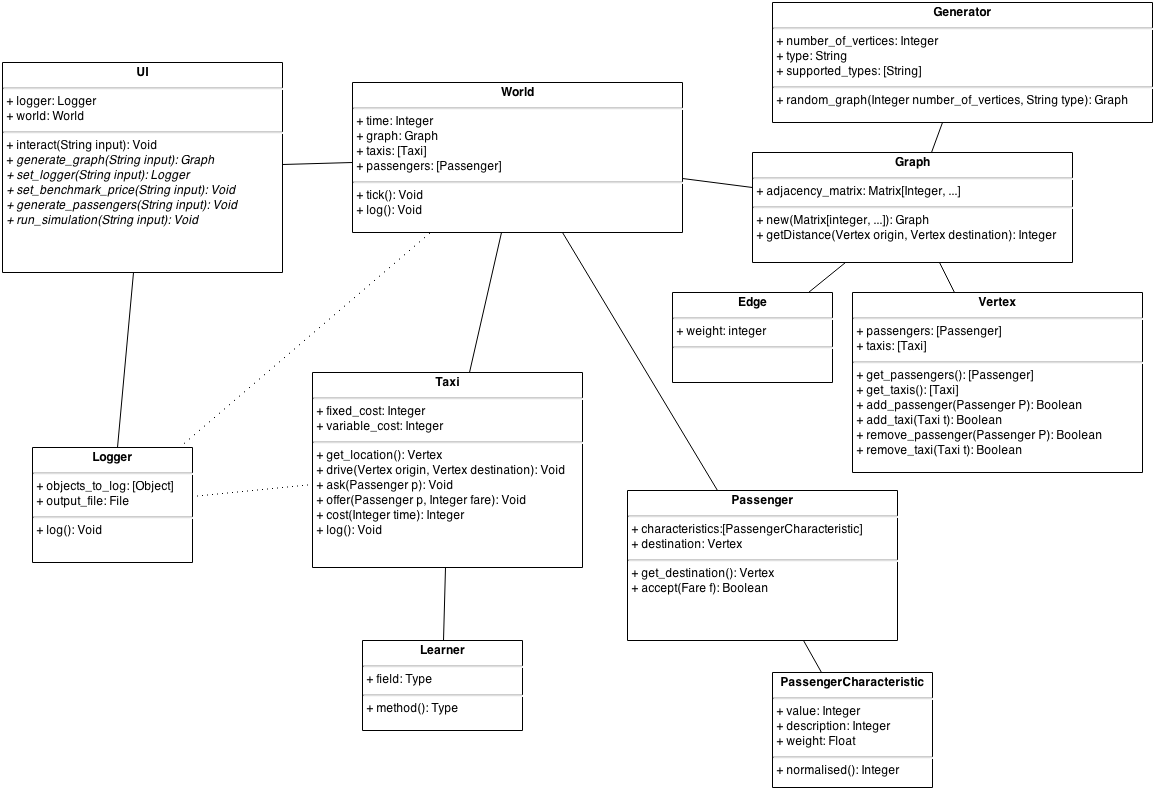
\includegraphics[width=\textwidth]{../figures/software_diagram}
    \caption{
      Software diagram
      \label{figure:design:software}
    }
  \end{center}
\end{figure}


How well does the implementation work? (as judged from the description in the
dissertation, and the demo)

What is the quality, sophistication and difficulty of the software (or
conceptual) implementation as judged from the description in the dissertation,
and the demo?

Is the programming (or modelling) style adequate and of good quality
(efficient, reusable, modular, clear code)?

Is the documentation in the code appropriate and useful?


\subsection{Implementation}

major system components, including main technologies

\todo{issues either here or in evaluation}


\subsubsection{Preliminaries}

automated virtualisation using vagrant, virtualbox, rvm for cross-platform
operation

Ruby, rubygems and bundler as the base

rspec and guard gems for supporting tdd. simplecov for code coverage to
identify any untested code (remark that this is no guarantee of correctness)

git for versioning


\subsubsection{User Interface}

rake and text file editing for simple user interface

runner for initialising and parsing input 


\subsubsection{The Environment}

world

Network: modelled using graphing library 'plexus'. It has not implemented an
algorithm to check for connectivity of directed graphs, therefore undirected
graphs are used.


\subsubsection{Learner}

characteristics, initialisation etc.

Q-learner algorithm


\subsubsection{Taxi}

taxi itself: characteristics, initialisation

state

action


(15, 3200 w)

Has the student carried out an evaluation?

Does the student present the results of the evaluation clearly and in a logical
manner?

Does the student explain the problems and difficulties found?

Does the student demonstrate an understanding and interpretation of results and
their significance?

Is there any critical evaluation of the project relative to the achievements of
related works?

Does the student present a personal reflection of what has been achieved and
not achieved in the project?

Has the student suggested future work?


\subsection{Future work}

Software related: fix the shortcomings identified above (TBD); extend to other learners, perhaps even non-MDP based

Socio-economical: evaluate the effect of deregulated prices on
passengers; effective way to model passengers


\newpage
\section{Conclusion}
\label{sec:conclusion}

This project was mostly successful in implementing a software simulation of a
taxi market where fare prices are chosen by a Q-Learner agent. 

The software fulfilled all of the core goals to the minimum specification, and
exceeded the minimum requirements in some areas. The software suffers from
several small implementation issues that have been clearly identified, and a
plan for fixing these issues was provided. While some problems were identified
with the software development approach that was followed, it was adequate and
proved beneficial overall.

The simulation experiment was successfully completed with six different
scenarios, testing different aspects of the system. It was found that having
variable fare pricing results in significantly larger profits to a taxi.
Furthermore, it was clear that the Q-Learner was a reasonable choice for
controlling the taxi and it's fare pricing as it showed a clear trend of
increasing profits over time.

However, the results additionally revealed an inconclusive profitability trend
for the Q-Learner in the fixed pricing simulation scenarios conducted for
benchmarking. This suggests that there may be a bug or a design oversight in
the software which will need fixing in future.

Nevertheless, variable pricing proved to be more profitable than fixed pricing,
therefore opening future possibilities for the project's topic and software.
Possible future work includes fixing the known issues with the software,
experimenting with different reinforcement learning strategies or even
researching the wider social implications of a variable fare pricing approach.
Beyond the realm of taxis, it is worth considering to utilise variable pricing
and reinforcement learning for public transport in general.


\newpage
\printbibliography

\appendix
(5, 500-1000 w?)

Is the manual written in a direct and easy to understand language?

Does the manual use task-oriented descriptions (e.g. “to open a file you click
on …”)?

Are there walk-through descriptions using detailed examples (e.g. “to enter
customer Joe Bloggs with Address …”)

What is the overall structure, layout, and use of pictures (where appropriate)?

\clearpage
\section{Maintenance Manual}

\todo{remove notes}

(5, 500-1000 w?)

Is there a description of the system and any third-party software required
including where to get it from?

Are there installation instructions and how good are they?

Is there a list of packages and files and what they are for?

Is there a description of how the system can be changed for most likely future
adaptations and extensions?

look at the 'projects' book for advice

\newpage
\section{Standard Simulation Run Analysis}
\label{sec:data:standard}

\includepdf[pages={-}]{../Data/standard/analysis.pdf}

\newpage
\section{Higher Benchmark Price Simulation Run Analysis}
\label{sec:data:higher_benchmark}

\includepdf[pages={-}]{../Data/higher_benchmark/analysis.pdf}

\newpage
\section{Lower Benchmark Price Simulation Run Analysis}
\label{sec:data:lower_benchmark}

\includepdf[pages={-}]{../Data/lower_benchmark/analysis.pdf}

\newpage
\section{Higher Price Range Simulation Run Analysis}
\label{sec:data:higher_range}

\includepdf[pages={-}]{../Data/higher_range/analysis.pdf}

\newpage
\section{Lower Price Range Simulation Run Analysis}
\label{sec:data:lower_range}

\includepdf[pages={-}]{../Data/lower_range/analysis.pdf}

\newpage
\section{Limited Time Simulation Run Analysis}
\label{sec:data:limited_time}

\includepdf[pages={-}]{../Data/limited_time/analysis.pdf}


\end{document}
